\clearpage
\section{Rezepte}

\subsection{Potenzrechnen}
\textbf{Kurzanleitung:}
\begin{enumerate}
	\item Gleichung aufschreiben $A^k=T^{-1} \cdot {A'}^k \cdot T$
	\item Eigenbasis aus n linear unabhängigen Eigenvektoren finden.
	\item Basis-Transformationsmatrix T berechnen.
	\item Diagonalisierte Matrix A' berechnen.
	\item $A^k$ berechnen.
\end{enumerate}
\textbf{Schritt für Schritt Anleitung:}
\begin{enumerate}
	\item Gleichung aufschreiben:\\
		$A^k=T^{-1} \cdot {A'}^k \cdot T\qquad A =\left(\begin{array}{cc}
			3 & 2\\
			1 & 2
		\end{array}\right)$
	\item Basis aus Eigenvektoren finden\\
		\begin{enumerate}
			\item Eigenwerte berechnen:
				$ det(A-\lambda E) = 0 \qquad \left|\begin{array}{cc}
				3-\lambda & 2\\
				1 & 2-\lambda
				\end{array}\right| = (3-\lambda)(2-\lambda)-1 \cdot 2 = 0 $\\[0.2cm]
				$= \lambda^2-5\lambda+4 = 0 \rightarrow (\lambda-1)(\lambda-4)=0 \rightarrow \lambda_1 = 1 \rightarrow \lambda_2 = 4$
			\item Eigenvektoren finden:\\
			\begin{minipage}{0.5\textwidth}
				$(A-\lambda_1 E)\cdot \vec{v_1} = 0$\\
				$\begin{array}{|cc|c|}
					\hline
					2 & 2 & 0\\
					1 & 1 & 0\\
					\hline
				\end{array} 
				\begin{array}{l}
				\rightarrow 2x_1 + 2y_1 = 0\\\rightarrow 1x_1 + 1y_1 = 0\end{array}
				\rightarrow\vec{v_1} = \left(\begin{array}{c} -1\\1 \end{array}\right)$
			\end{minipage}
			\begin{minipage}{0.5\textwidth}
				$(A-\lambda_2 E)\cdot \vec{v_2} = 0$\\
				$\begin{array}{|cc|c|}
				\hline
				-1 & 2 & 0\\
				1 & -2 & 0\\
				\hline
				\end{array} 
				\begin{array}{l}
				\rightarrow -1x_2 + 2y_2 = 0\\\rightarrow 1x_2 - 2y_1 = 0\end{array}
				\vec{v_2} = \left(\begin{array}{c} 2\\1 \end{array}\right)$
			\end{minipage}
		\end{enumerate}
	\item $T$ und $T^{-1}$ berechnen:\\[0.2cm]
		\begin{minipage}
			{0.5\textwidth}$T^{-1}=(\vec{v_1} \quad \vec{v_2}) = \left(\begin{array}{cc}-1 & 2 \\ 2 & 1\end{array}\right)$
		\end{minipage}
		\begin{minipage}{0.5\textwidth}
			$T=T^{-1^{-1}}= (\vec{v_1} \quad \vec{v_2})^{-1} = \displaystyle \frac 1 3 \left(\begin{array}{cc}-1 & 2 \\ 1 & 1\end{array}\right)$
		\end{minipage}
	\item Diagonal Matrix A' berechnen:\\
		$A' = \left(\begin{array}{cc} \lambda_1 & 0\\ 0 & \lambda_2 \end{array}\right) = \left(\begin{array}{cc} 1 & 0\\ 0 & 4 \end{array}\right)$
		
	\item $A^k$ berechnen:\\
		$A^k=T^{-1} \cdot {A'}^k \cdot T = 
		\left(\begin{array}{cc}-1 & 2 \\ 2 & 1\end{array}\right) \cdot
		\left(\begin{array}{cc} 1^k & 0\\ 0 & 4^k \end{array}\right) \cdot
		\displaystyle \frac 1 3 \left(\begin{array}{cc}-1 & 2 \\ 1 & 1\end{array}\right)$
\end{enumerate}
\clearpage
\subsection{Kameraabbildungen}

\subsubsection{Bildpunkt zum 3D Punkt}
\textbf{Gegeben:}\\
\begin{tabular}{llcll}
	Brennweite: & $f=100$pixel &\quad& Bild grösse: & $m_x \cdot m_y =120 \cdot 90$\\
	Position Kameras: & $C_1=(100;0;0) \quad C_2=(0;100;0)$ && Bildpunkte: & $B_1=(36;40) \quad B_2=(65;58)$\\
	Drehmatrix $D_1$: & $D_1=\left(\begin{array}{ccc} 
	0 & -1 & 0\\
	0 & 0 & 1\\
	-1 & 0 & 0 
	\end{array}\right)  $ && Drehmatrix $D_2$: & $D_2=\left(\begin{array}{ccc} 
	0 & 0 & -1\\
	1 & 0 & 0\\
	0 & -1 & 0 
	\end{array}\right)  $
\end{tabular}\\[0.4cm]
\textbf{Gesucht:} Punkt $Q$ welche auf den Bildpunkten $B_1$ \& $B_2$ dargestellt ist.\\
\begin{enumerate}
	\item Kameramatrix aufstellen\\
		$K=\left(\begin{array}{ccc}
			f & 0 & mx/2\\
			0 & f & my/2\\
			0 & 0 & 1
		\end{array}\right) = \left(\begin{array}{ccc}
		100 & 0 & 60\\
		0 & 100 & 45\\
		0 & 0 & 1
		\end{array}\right)$
	\item Eine Gerade pro Kamera berechnen mit je einem $\vec{c_i}$ = Stützvektor und einem Richtungsvektor\\ $\vec{r_i}=(KD_i)^{-1}\cdot \vec{\tilde{b_i}} \rightarrow \vec{\tilde{b_i}} = \vektor{b_{ix}}{b_{iy}}{1}$\\
	\begin{equation*}
	\vec{r_1}=(KD_1)^{-1}\cdot \vec{\tilde{b_1}} =
	\left[\left(\begin{array}{ccc}
	100 & 0 & 60\\
	0 & 100 & 45\\
	0 & 0 & 1
	\end{array}\right)
	\left(\begin{array}{ccc}
	0 & -1 & 0\\
	0 & 0 & 1\\
	-1 & 0 & 0 
	\end{array}\right)\right]^{-1}\cdot
	\vektor{36}{60}{1}=\vektor{-1.00}{" "0.24}{-0.05}
	\end{equation*}\\
	\begin{equation*}
	\vec{r_2}=(KD_2)^{-1}\cdot \vec{\tilde{b_2}} =
	\left[\left(\begin{array}{ccc}
	100 & 0 & 60\\
	0 & 100 & 45\\
	0 & 0 & 1
	\end{array}\right)
	\left(\begin{array}{ccc}
	0 & 0 & -1\\
	1 & 0 & 0\\
	0 & -1 & 0 
	\end{array}\right)\right]^{-1}\cdot
	\vektor{65}{58}{1}=\vektor{" "0.13}{-1.00}{-0.05}
	\end{equation*}
	\begin{minipage}{0.5\textwidth}
		$\vec{p_1} = \vec{c_1}+t \cdot \vec{r_1}= \vektor{100}{0}{0}+t\cdot \vektor{-1.00}{" "0.24}{-0.05}$
	\end{minipage}
	\begin{minipage}{0.5\textwidth}
		$\vec{p_2} = \vec{c_2}+s \cdot \vec{r_2}= \vektor{0}{100}{0}+t\cdot \vektor{" "0.13}{-1.00}{-0.05}$
	\end{minipage}
	\item Matrix Gleichung aufstellen\\
		$\underbrace{\left(\begin{array}{ccccc}
			" "&" "&" "&" "& 0\\
			" "& E &" "&-\vec{r_1}&0\\
			" "&" "&" "&" "& 0\\
			" "&" "&" "& 0 & " "\\
			" "& E &" "& 0 &-\vec{r_2}\\
			" "&" "&" "& 0 & " "
		\end{array}\right)}_{\displaystyle A}\cdot
		\underbrace{\left(\begin{array}{c}
		x\\y\\z\\t\\s
		\end{array}\right)}_{\displaystyle\vec{x}} = 
		\underbrace{\left(\begin{array}{c}
		" "\\\vec{c_1}\\" "\\" "\\\vec{c_2}\\" "
		\end{array}\right)}_{\displaystyle\vec{b}} \rightarrow 
		\left(\begin{array}{ccccc}
			1 & 0 & 0 &" "1.00& 0\\
			0 & 1 & 0 &  -0.24& 0\\
			0 & 0 & 1 &" "0.05& 0\\
			1 & 0 & 0 & 0 &  -0.13\\
			0 & 1 & 0 & 0 &" "1.00\\
			0 & 0 & 1 & 0 &" "0.05
		\end{array}\right)\cdot
		\left(\begin{array}{c}
			x\\y\\z\\t\\s
		\end{array}\right) = 
		\left(\begin{array}{c}
			100\\0\\0\\0\\100\\0
		\end{array}\right)$
		
	\item Least-Square verfahren\\[0.2cm]
		$A^t \cdot A \cdot \vec{x} = A^t \cdot \vec{b}$\\
		$\vec{x}=(A^t \cdot A)^{-1} \cdot A^t \cdot \vec{b} \rightarrow$ In TR eingeben $\rightarrow \underline{\underline{Q=(x;y;z)}}$ 
\end{enumerate}


\subsubsection{3D-Punkt zu Bildpunkt}
\textbf{Gegeben:}\\
\begin{tabular}{llcll}
	Brennweite: & $f=500$pixel &\quad& Bild grösse: & $m_x \cdot m_y =640 \cdot 480$\\
	Position Kamera: & $C=(-300;0;200)$ && Punkt im Raum: & $Q=(50;100;450)$\\
	Drehmatrix: &$D=\left(\begin{array}{ccc} 
	\frac 1 2 & 0 & -\frac{\sqrt{3}}{2}\\
	0 & 1 & 0\\
	\frac{\sqrt{3}}{2} & 0 & \frac{1}{2} 
	\end{array}\right)  $
\end{tabular}\\[0.2cm]
\textbf{Gesucht:}\\
Bildpunkt B auf welchem sich der Punkt Q befindet.\\
\begin{enumerate}
	\item Kameraprojektionsmatrix berechnen:\\
		\begin{equation*}
			P = KD(E-\vec{x}) = 
			\left(\begin{array}{ccc} 
			500 & 0 & 320\\
			0 & 500 & 240\\
			0 & 0 & 1 
			\end{array}\right)
			\cdot
			\left(\begin{array}{ccc} 
			\frac 1 2 & 0 & -\frac{\sqrt{3}}{2}\\
			0 & 1 & 0\\
			\frac{\sqrt{3}}{2} & 0 & \frac{1}{2} 
			\end{array}\right)
			\cdot
			\left(\begin{array}{cccc} 
			1 & 0 & 0 & 300\\
			0 & 1 & 0 & 0\\
			0 & 0 & 1 & -200
			\end{array}\right)
			=
			\left(\begin{array}{cccc} 
			527.128 & 0 & -273.013 & 212741\\
			207.846 & 500 & 120 & 38353.8\\
			0.866025 & 0 & 0.5 & 159.808
			\end{array}\right)			
		\end{equation*}
		
	\item Homogener Bildpunkt berechnen
	\begin{equation*}
		\tilde{b} = P \cdot \tilde{q}
		=
		\left(\begin{array}{cccc} 
		527.128 & 0 & -273.013 & 212741\\
		207.846 & 500 & 120 & 38353.8\\
		0.866025 & 0 & 0.5 & 159.808
		\end{array}\right)
		\cdot
		\left(\begin{array}{c}
		50\\100\\450\\1
		\end{array}\right)
		=
		\vektor{116242}{152746}{428.109}
	\end{equation*}
	
	\item Bildpunkt berechnen\\
	Durch den dritten Komponenten Teilen\\
	\begin{equation*}
		\vec{b}
		=
		\left(\begin{array}{c}
			\displaystyle \frac{116242}{428.109}\\
			" "\\
			 \displaystyle \frac{152746}{428.109}
		\end{array}\right)
		= 
		\underline{\underline{
				\left(\begin{array}{c}
				271.524\\
				356.793
				\end{array}\right)}}
	\end{equation*}
\end{enumerate}
\clearpage
\subsection{Kugelprojektionen}
	\begin{minipage}{0.4\textwidth}
		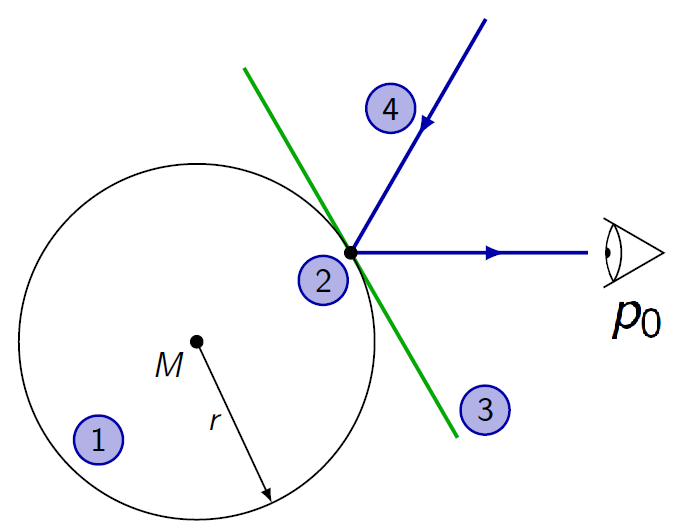
\includegraphics[width=\textwidth]{pics/Kugelprojektion.png}
	\end{minipage}
	\begin{minipage}{0.6\textwidth}
		\begin{enumerate}
			\item Gleichung für Kugel
			\item Durchstosspunkt
			\item Tangentialebene (Falls relevant)
			\item Reflektierter Strahl
		\end{enumerate}
	\end{minipage}\\
	\begin{enumerate}
		\item Kugelgleichung:
			\begin{equation*}
				(\vec{p} - \vec{m})\bullet (\vec{p} - \vec{m}) = r^2
			\end{equation*}
		\item Durchstosspunkt berechnen:\\
			Geradengleichung $\vec{p} = \vec{p_0} + s \cdot \vec{r}$ in Kugelgleichung einsetzen:\\
			\begin{tabular}{ll}
				$p_0 = $ Ortsvektor von Punkt $P_0$ & $\vec{r} = $ Richtungsvektor 
			\end{tabular}
			\begin{equation*}
			(\vec{p_0} + s \cdot \vec{r} - \vec{m})\bullet (\vec{p_0} + s \cdot \vec{r} - \vec{m}) = r^2
			\end{equation*}
			\begin{equation*}
			((\vec{p_0}-\vec{m}) + s \cdot \vec{r}) 
			\bullet
			((\vec{p_0}-\vec{m}) + s \cdot \vec{r}) = r^2
			\end{equation*}
			\begin{equation*}
			s^2 \cdot (\vec{r} \bullet \vec{r}) +
			s\cdot(2 \cdot (\vec{p_0}-\vec{m}) \bullet \vec{r}) +
			(\vec{p_0}-\vec{m}) \bullet (\vec{p_0}-\vec{m})
			-r^2 = 0
			\qquad \rightarrow \qquad
			s_{1/2} = \displaystyle \frac{-b \pm \sqrt{b^2-4ac}}{2a}
			\end{equation*}
			Es muss nun das kleinere  $s$ gewählt werden da mit diesem s der Durchstosspunkt welcher näher bei $P_0$ liegt gefunden wird.\\
			Nun muss der Punkt $P_1$ berechnet werden dazu muss $s$ in die Geradengleichung eingesetzt werden.
			\begin{equation*}
			\vec{p_1} = \vec{p_0} + s_1 \cdot \vec{r}
			\end{equation*}
						
		\item Reflektierter Strahl berechnen\\
		Zuerst muss der Normalenvektor der Tangentialebene bestimmt werden. Dieser geht von $P_1$ nach $M$ und hat die Länge $r$:\\
		\begin{equation*}
			\vec{n} = \vec{m} -\vec{p_1}
		\end{equation*}
		Nun muss der Richtungsvektor $\vec{r}$ in $\vec{r_\perp}$ und in $\vec{r_\parallel}$ aufgeteilt werden:\\
			\begin{minipage}{0.5\textwidth}
			\begin{equation*}
			\vec{r_\perp} = \displaystyle \frac{\vec{r} \bullet \vec{n}}{|\vec{n}|} \cdot
			\displaystyle \frac{\vec{n}}{|\vec{n}|}
			= \displaystyle \frac{\vec{r} \bullet \vec{n}}{r^2} \cdot \vec{n}
			\end{equation*}
			\begin{equation*}
			\vec{r_\parallel} = \vec{r} - \vec{r_\perp}
			\end{equation*}
			\begin{equation*}
			\vec{r'} = \vec{r_\parallel} - \vec{r_\perp} =
			\vec{r} - 2 \cdot \vec{r_\perp} =
			\vec{r} -2 \cdot \displaystyle \frac{\vec{r} \bullet \vec{n}}{r^2} \cdot \vec{n}
			\end{equation*}
			\end{minipage}
		\begin{minipage}{0.5\textwidth}
			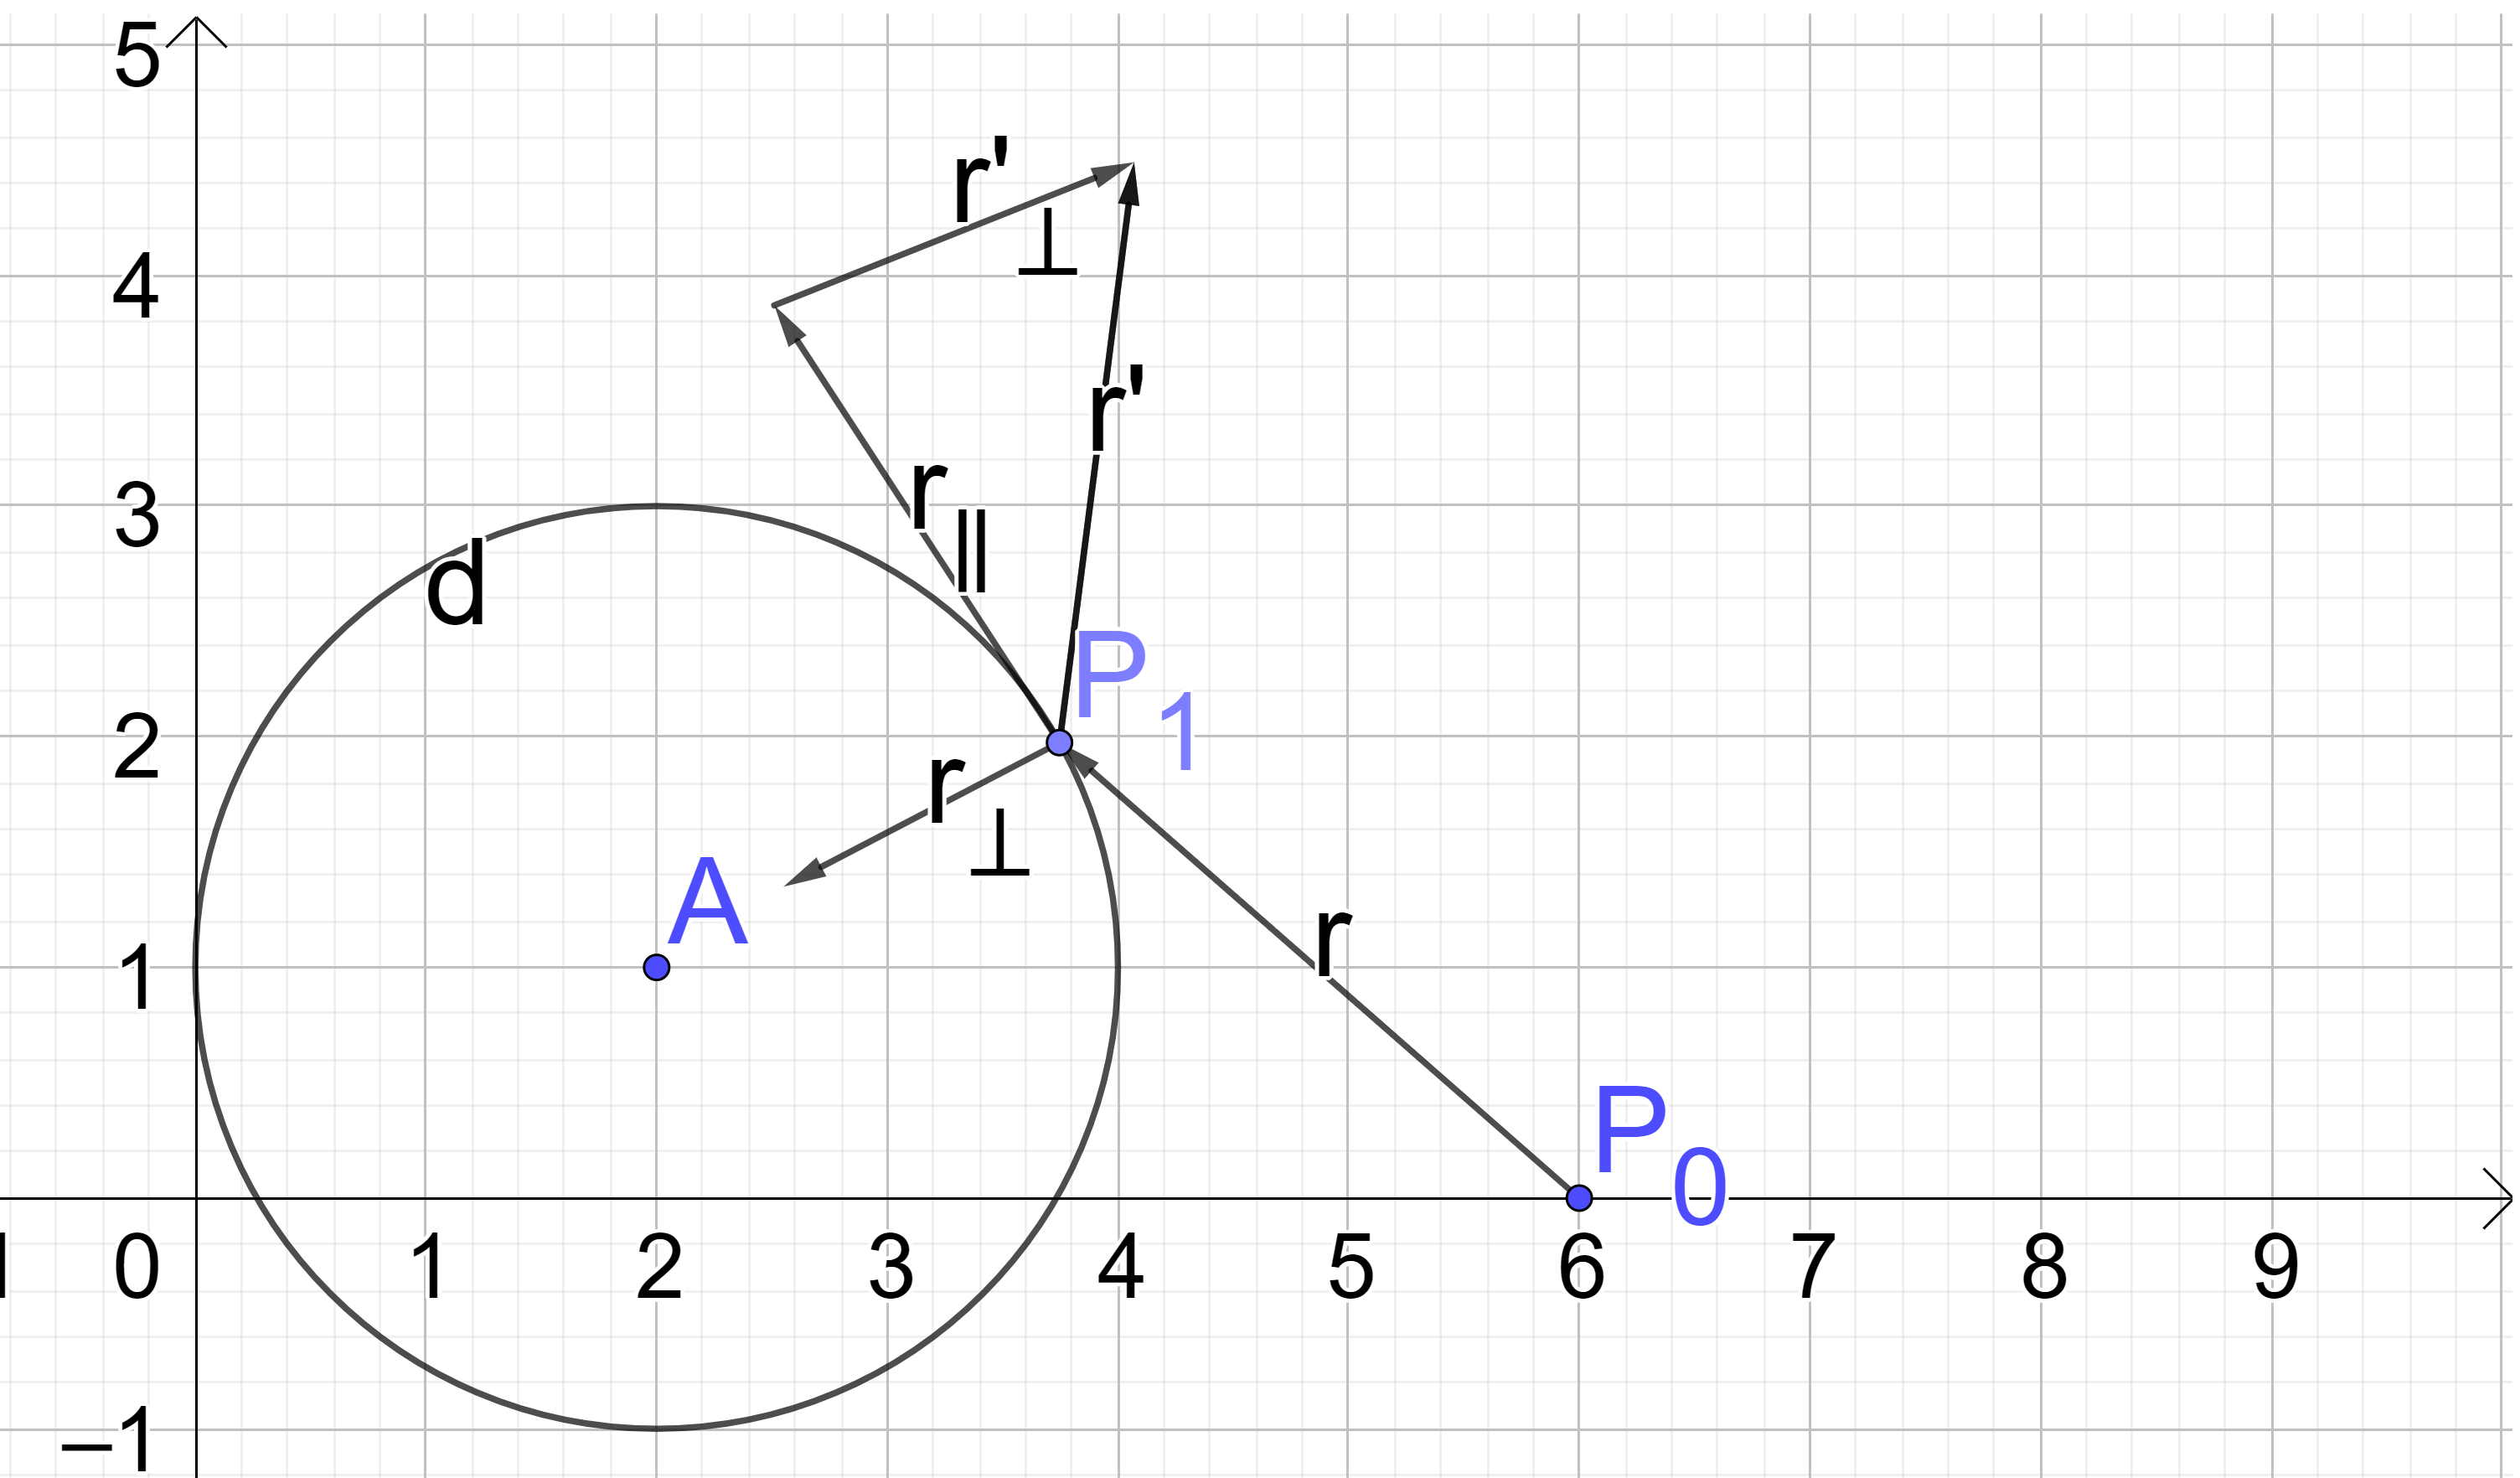
\includegraphics[width=\textwidth]{pics/Kugelprojektion_2.png}
		\end{minipage}
	
	\item Tangentialebene
		Wenn nun doch die Tangentialebene berechnet werden muss kann dies mit einer der folgenden Formeln gemacht werden
		\begin{itemize}
			\item $(\vec{p} - \vec{p_1}) \bullet (\vec{p_1} - \vec{m}) = 0 \qquad \qquad \vec{p} =$ Punkt auf Ebene
			\item $(\vec{p}-\vec{m}) \bullet (\vec{p_1} - \vec{m})=r^2$
		\end{itemize}
	\end{enumerate}
